\chapter{Progettazione di un sistema Embedded}
\section{Analisi dei requisiti}
\subsection{Requisiti funzionali}
Il sistema realizzato deve permettere ad uno o più giocatori di competere per sbloccare dei lucchetti. Ad ogni lucchetto sbloccato si supera il livello fino a quando i livelli non terminano e il gioco si dice finito. Durante il gioco sono presenti delle penalità e dei bonus.

\subsection{Requisiti non funzionali}
Le performance utili per la buona riuscita del progetto a cui non si può rinunciare riguardano la rilevazione della distanza e l'invio dei feedback locali/remoti.
Il tempo gioca un ruolo importante in questo progetto, quindi si devono evitare inutili ritardi nella rilevazione ed invio delle informazioni.

\newpage
\section{Casi d'uso}
\subsection{Caso d'uso 1}
\begin{figure}[!ht]
	\centering
	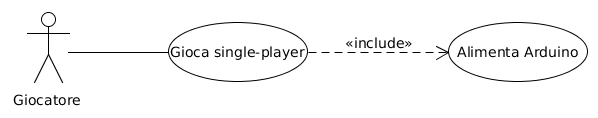
\includegraphics[scale=.4]{img/UML/UseCases/case1.png}
	\caption{Caso d'uso 1}
\end{figure}
\begin{table}[]
	\centering
	\caption{Caso d'uso 1}
	\begin{tabular}{ll}
		\textbf{ID}                                          & UC1                                                                                                                                                                                                                                            \\ \hline
		\multicolumn{1}{|l|}{\textbf{ATTORI}}                & \multicolumn{1}{l|}{Giocatore}                                                                                                                                                                                                                 \\ \hline
		\multicolumn{1}{|l|}{\textbf{PRECONDIZIONI}}         & \multicolumn{1}{l|}{Il giocatore vuole iniziare una partita single player}                                                                                                                                                                      \\ \hline
		\multicolumn{1}{|l|}{\textbf{SEQUENZA DEGLI EVENTI}} & \multicolumn{1}{l|}{\begin{tabular}[c]{@{}l@{}}1. Il caso d'uso inizia quando un giocatore vuole giocare a Jimmy Challenge.\\ 2. Il giocatore deve alimentare l'Arduino per poter giocare.\\ 3. Il programma inizia ad eseguire.\end{tabular}} \\ \hline
		\multicolumn{1}{|l|}{\textbf{POSTCONDIZONI}}         & \multicolumn{1}{l|}{1. Il giocatore gioca.}                                                                                                                                                                                                    \\ \hline
	\end{tabular}
\end{table}

\newpage
\subsection{Caso d'uso 2}
\begin{figure}[!ht]
	\centering
	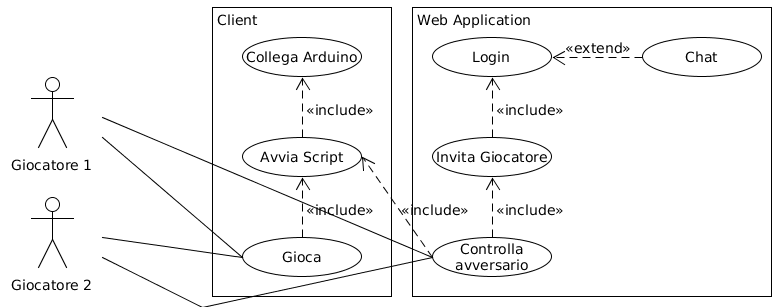
\includegraphics[scale=.4]{img/UML/UseCases/case2.png}
	\caption{Caso d'uso 2}
\end{figure}
\begin{table}[]
	\centering
	\caption{Caso d'uso 2}
	\begin{tabular}{ll}
		\textbf{ID}                                          & UC2                                                                                                                                                                                                                                                                                                                                                                                                                                                                                                                                                                                  \\ \hline
		\multicolumn{1}{|l|}{\textbf{ATTORI}}                & \multicolumn{1}{l|}{Giocatore 1, Giocatore 2}                                                                                                                                                                                                                                                                                                                                                                                                                                                                                                                                        \\ \hline
		\multicolumn{1}{|l|}{\textbf{PRECONDIZIONI}}         & \multicolumn{1}{l|}{I due attori vogliono giocare una partita a Jimmy Challenge multiplayer online.}                                                                                                                                                                                                                                                                                                                                                                                                                                                                                 \\ \hline
		\multicolumn{1}{|l|}{\textbf{SEQUENZA DEGLI EVENTI}} & \multicolumn{1}{l|}{\begin{tabular}[c]{@{}l@{}}1. Il caso d'uso inizia quando i due giocatori vogliono giocare online e si collegano al sito.\\ 2. I giocatori devono collegare al PC l'Arduino.\\ 3. I giocatori devono far avviare lo script in Python per inviare i dati al server.\\ 4. I giocatori devono effettuare l'accesso al sito.\\ 5. I giocatori possono chattare.\\ 6. I giocatori devono invitarsi ad iniziare una nuova partita.\\ 7. I giocatori iniziano a giocare.\\ 8. Ogni giocatore può controllare lo stato della partita dell'altro giocatore.\end{tabular}} \\ \hline
		\multicolumn{1}{|l|}{\textbf{POSTCONDIZONI}}         & \multicolumn{1}{l|}{1. I due giocatori giocano.}                                                                                                                                                                                                                                                                                                                                                                                                                                                                                                                                     \\ \hline
	\end{tabular}
\end{table}

\newpage
\section{Modeling}
Il sistema si suddivide in più parti:
\begin{itemize}
	\item parte fisica lato client/server;
	\item parte software lato client/server;
	\item networking lato client/server.
\end{itemize}

\subsection{Modellazione della parte fisica - lato client}
Dal punto di vista fisico, si ha un Arduino UNO:
\begin{itemize}
	\item connesso ad una breadboard e a dei componenti hardware attraverso i sui pin digitali
	\item connesso ad un PC mediante la porta USB (da cui riceve l'alimentazione a 5v). 
\end{itemize}
Ogni componente della breadboard ha un proprio impiego e può essere distinto in \textbf{sensore} ed \textbf{attuatore} secondo la visione di \textit{sistema reattivo}.

	\begin{quote}
		\textbf{Reactive system}: è l’ambiente esterno che determina gli eventi che	condizionano l’esecuzione del sistema
	\end{quote}	
La connessione seriale via USB serve per inviare i dati campionati dall'Arduino verso il PC. A loro volta questi dati possono servire per creare una interfaccia utente locale (per esempio su terminale) o remota, su browser.

\subsection{Modellazione della parte logica - lato client}
Per realizzare il comportamento dinamico del progetto, nella parte software si è replicato il funzionamento di una macchina a stati finiti (\textit{FSM}) che esegue dei task.

	\begin{quote}
		\textbf{Macchine a stati finiti} (o \textbf{\textit{automi a stati finiti}}): sono il modello nel discreto più utilizzato per modellare sistemi embedded.
		
		Ogni FSM opera in una sequenza di passi (discreti) e la sua dinamica è caratterizzata da sequenze di eventi (discreti).
		
		Un evento discreto avviene ad un determinato istante e non ha durata.
	\end{quote}
	
	\begin{quote}
		\textbf{Decomposizione in task}: principio di progettazione importante, rende modulare il sistema in quanto:
		\begin{itemize}
			\item ogni modulo è rappresentato da un task (compito da eseguire)
			\item un task può essere decomposto in sotto-task in modo ricorsivo o un task complesso può essere definito come composizione di sotto-task più semplici
		\end{itemize}
		Vantaggi:
		\begin{itemize}
			\item separation of concerns
			\item l'utilizzo di singoli moduli per una migliore comprensibilità del comportamento
			\item debugging semplificato
			\item supporto alla modificabilità, all'estensione ed al riuso del codice
		\end{itemize}
	\end{quote}	
Si è fatto uso della programmazione ad oggetti, modellando ogni task (es. \textit{LedTask}, \textit{BuzzerTask}, etc.) come una classe separata che estende la classe base \textit{Task}. In ogni \textit{task} viene fatto l'\textbf{\textit{inject} del comportamento} da avere.\\
La simulazione della sensazione di lavorare su un sistema multi-tasking e cooperativo è realizzata tramite una schedulazione \textbf{round-robin} dei vari task. È stato necessario quindi introdurre uno \textit{Scheduler} per richiamare ciclicamente le funzioni \textit{tick()} dei vari task.

\begin{itemize}	
	\item si è fatto uso della programmazione Object-Oriented per rendere la struttura del codice ingegneristica, lineare e scalabile;
	\item si sono utilizzate le lambda expression per definire il comportamento di ogni task.
\end{itemize}
La comunicazione tra i task avviene attraverso variabili condivise. Queste variabili appartengono alla classe Context.\\
Per quanto riguarda la connessione USB, per scelta progettuale, tutti i dati inviati dall'Arduino al PC sono formattati in \textbf{JSON}.

\subsection{Modellazione della parte fisica - lato server}
A lato server si ha un Odroid C2 (prodotto da \href{http://www.hardkernel.com/main/main.php}{Hardkernel}) con sistema operativo Arch Linux ARM:
\begin{itemize}
	\item CPU: ARM Cortex-A53 Quad Core 2GHz;
	\item RAM: 2GB DDR3;
	\item 40pin GPIOs + 7pin I2S;
	\item Gigabit Ethernet;
	\item 4 x USB 2.0.
\end{itemize}
Il dispostivo è collegato in rete e funge da server per abilitare la modalità multiplayer di Jimmy Challenge dalla parte client tramite lo script python in esecuzione sul dispositivo collegato all'Arduino.\\
In un'ottica più orientata all'hardware, al server è collegato un LCD 16x2 che mostra alcune statistiche sullo stato attuale dei servizi e delle risorse.

Lo schema \ref{img:server} presenta il monitor LCD collegato ai pin GPIO del Odroid con un potenziometro per l'aggiustamento del contrasto.\\
Al fine di collegare in rete il server si è aggiunto un modulo WiFi (TP-Link TL-WN722N) tramite una porta USB.

\subsection{Modellazione della parte logica - lato server}
Per permettere agli utenti di giocare tra di loro online, il server mette a disposizione:
\begin{itemize}
	\item una interfaccia per visualizzare gli utenti loggati;
	\item una chat globale in cui poter invitare gli utenti a giocare;
	\item una view con lo stato del gioco.
\end{itemize}
La piattaforma riceve messagi JSON dallo script lato client tramite richieste POST ad un'interfaccia PHP RESTful. Una volta che le informazioni sono inviate al server, sono elaborate e pubblicate ai vari subscriber tramite Server-Sent Events (sempre utilizzando JSON come modello).\\
La modalità multiplayer di Jimmy Challenge in sostanza consiste in una applicazione web, quasi real-time, in cui i giocatori possono vedere, tramite l'apposita view, lo stato e l'avanzamento dell'avversario nel gioco.\\
Per garantire massime performance e sicurezza sono state adottate queste tecnologie:
\begin{itemize}
	\item \textbf{NGINX} come web server;
	\item \textbf{PHP 7} come backend e motore delle parti dinamiche dell'applicazione e che implementa l'interfaccia RESTfull;
	\item \textbf{Javascript} per elaborazione lato client;
	\item \textbf{MySQL} per lo store degli account degli utenti;
	\item \textbf{Redis} come staging area per i dati temporanei da condividere con \textbf{tutti} i subscriber;
	\item \textbf{JSON} come modello per i messaggi scambiati;
	\item \textbf{HTTPS} over TLS
	\item \textbf{JSON Web Signature} per i token JWS
\end{itemize}
Il monitor LCD visualizza alcune statistiche sulle risorse usate dal sistema:
\begin{itemize}
	\item RAM usata;
	\item Spazio disco usato della partizione di root ('/');
	\item Temperatura e percentuale di carico della CPU;
	\item Indirizzo IP interno;
	\item Traffico in upload e in download.
\end{itemize}
I dati stampati sullo schermo LCD sono collezionati e formattati tramite uno script python che utilizza un wrapper del porting di \href{https://github.com/hardkernel/WiringPi2-Python}{WiringPi} per i dispotivi Odroid.

\section{Design}
Il sistema si suddivide in più aree:
\begin{enumerate}
	\item connessione USB da Arduino UNO verso il PC;
	\item I/O locale attraverso Arduino UNO;
	\item input per invio dei dati seriali al server attraverso Python;
	\item connessione del PC ad un server;
	\item feedback remoto su browser;
	\item sito internet come GUI remota;
	\item gestione del server remoto.
\end{enumerate}

\section{Analysis}
Potenzialità software di Arduino UNO sfruttate:
\begin{itemize}
	\item programmazione Object-Oriented con \href{https://it.wikipedia.org/wiki/Wiring}{Wiring \footnote{Wiring - linguaggio di programmazione semplice e intuitivo derivato dal C e dal C++}}.
	\begin{itemize}
		\item modularizzazione in classi;
		\item utilizzo di oggetti e metodi;
		\item information hiding;
		\item ereditarietà;
		\item polimorfismo.
	\end{itemize}
	\item utilizzo di \textit{lambda expressions}
\end{itemize}
Potenzialità hardware di Arduino UNO sfruttate:
\begin{itemize}
	\item sono stati utilizzati tutti i 12 pin di I/O digitale;
	\item si è cercato di limitare l'utilizzo di \textbf{delay} per mantenere le prestazioni ottimali;
	\item in alcuni casi al posto dei \textit{delay} si è fatto ricorso a dei \textbf{custom timer} impiegando il metodo \textbf{millis()};
\end{itemize}